\chapter{Espacios M\'etricos, Coberturas y Complejos Simpliciales}

Debido a que las caracter\'isticas topol\'ogicas y geom\'etricas suelen ser asociadas con espacios continuos,
datos representados como una conjunto finito de observaciones no revelan informaci\'on topol\'ogica
directamente. Una manera natural de revelar alg\'un tipo de estructura topol\'ogica en los datos
es ``conectar'' puntos de datos que se encuentren cerca con el prop\'osito de exhibir una forma continua
global subyacente en los datos. Usualmente cuantificamos la noci\'on de cercania entre puntos utilizando
una distancia (o medida de disimilaridad), y muchas veces resulta conveniente considerar conjuntos de datos
como espacios m\'etricos discretos o muestras de espacios m\'etricos. Esta secci\'on introduce conceptos
generales para la inferencia geom\'etrica y topol\'ogica; una presentaci\'on m\'as completa del tema se
encuentra en el estudio por Boissonnat et al. (2018) \cite{Boissonnat2018}.

\section*{Espacios M\'etricos}

Recordemos que un espacio m\'etrico $\left(M, \rho\right)$ es un conjunto $M$ con una funci\'on
$\rho: M \times M \rightarrow \mathbb{R}_{+}$, llamada distancia, tal que para cualquier $x, y, z \in M$,
se tiene lo siguiente:

\begin{enumerate}[label=\roman*)]
    \item $\rho\left(x, y\right) \geq 0$ y $\rho\left(x, y\right) = 0$ si y s\'olo si $x = y$,
    
    \item $\rho\left(x, y\right) = \rho\left(y, x\right)$, y
    
    \item $\rho\left(x, z\right) \leq \rho\left(x, y\right) + \rho\left(y, z\right)$.
    
\end{enumerate}

Dado un espacio m\'etrico $\left(M, \rho\right)$, el conjunto de subconjuntos compactos de
$\left(M, \rho\right)$ denotado por $\mathcal{K}\left(M\right)$, puede ser dotado
con la distancia de Hausdorff; dados dos subconjuntos compactos $A, B \subseteq M$,
la distancia de Hausdorff $d_{H}\left(A, B\right)$ entre $A$ y $B$ es
definida como el n\'umero no negativo m\'as peque\~{n}o $\delta$, tal que para cualquier $a \in A$, existe
$b \in B$ de manera que $\rho\left(a, b\right) \leq \delta$ (Figura \ref{fig:Figura 1}). En otras palabras,
si dado cualquier subconjunto compacto $C \subseteq M$, denotamos por $d\left(\cdot, C\right):
M\rightarrow\mathbb{R}_{+}$ a la funci\'on distancia de $C$ definida por
$d\left(x, C\right) \coloneqq \inf_{c\in C}\rho\left(x, c\right)$ para cualquier $x \in M$, entonces se
puede probar que la distancia de Hausdorff entre $A$ y $B$ esta definida por una de las siguientes
igualdades:

\begin{align*}
    d_{H}\left(A, B\right) & = \max\left\{\sup_{b\in B}d\left(b, A\right),
    \sup_{a\in A}d\left(a, B\right)\right\} \\
    & = \sup_{x\in M}\left|d\left(x, A\right) - d\left(x, B\right)\right| =
    \left\|d\left(\cdot, A\right) - d\left(\cdot, B\right)\right\|_{\infty}
\end{align*}

Es un resultado cl\'asico que la distancia de Hausdorff es en efecto una distancia en el conjunto de
subconjuntos compactos de un espacio m\'etrico. Desde la perspectiva del ATD, esta distancia
brinda una manera conveniente de cuantificar la proximidad entre diferentes conjuntos de datos que
provienen del mismo espacio m\'etrico. Sin embargo, a veces es necesario comparar conjuntos de datos que
no son muestreados del mismo espacio. Por fortuna la noci\'on de la distancia de Hausdorff puede ser
generalizada para comparar cualquier par de espacios m\'etricos compactos, esta es la idea de la distancia
de Gromov-Hausdorff.

Dados dos espacios m\'etricos compactos, $\left(M_{1}, \rho_{1}\right)$ y $\left(M_{2}, \rho_{2}\right)$,
decimos que son isom\'etricos si existe una biyecci\'on $\phi: M_{1}\rightarrow M_{2}$ que preserva
distancias, esto es, $\rho_{2}\left(\phi\left(x\right), \phi\left(y\right)\right) =
\rho_{1}\left(x, y\right)$ para cualquier $x, y \in M_{1}$. La distancia de Gromov-Hausdorff mide cuan lejos
est\'an dos espacios m\'etricos de ser isom\'etricos.

\begin{definicion}
    La distancia de Gromov-Hausdorff $d_{GH}\left(M_{1}, M_{2}\right)$ entre dos espacios m\'etricos
    compactos es el \'infimo de los n\'umeros reales $r \geq 0$ tal que existe un espacio m\'etrico
    $\left(M, \rho\right)$ y dos subespacios compactos $C_{1}$ y $C_{2} \subset M$ que son isom\'etricos
    a $M_{1}$ y $M_{2}$ y que cumplen $d_{H}\left(C_{1}, C_{2}\right) \leq r$.
\end{definicion}

\begin{figure}[h]
    \centering
    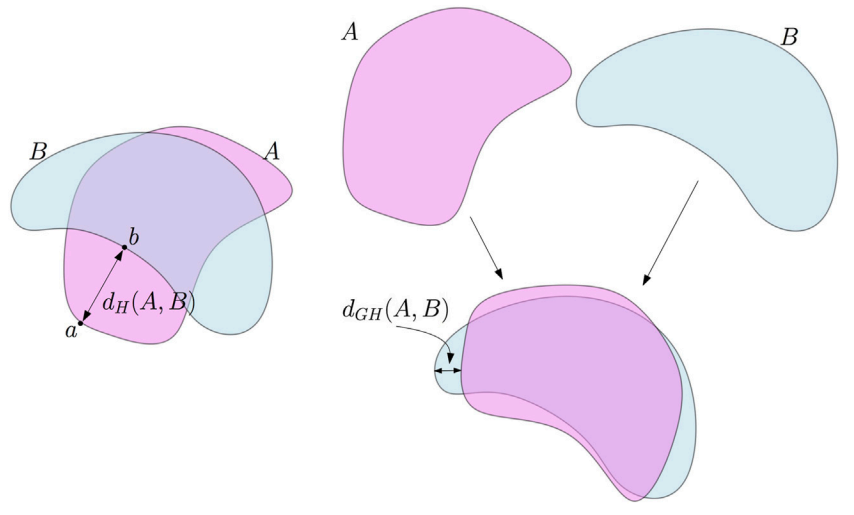
\includegraphics[width=0.85\linewidth]{./figures/Figura1_c1.png}
    \caption{
        Izquierda: la distancia de Hausdorff entre dos subconjuntos $A$ y $B$ en el plano. en este ejemplo,
        $d_{H}\left(A, B\right)$ es la distancia entre el punto $a$ en $A$ que es el m\'as lejano a $B$ y
        su vecino m\'as cercano $b$ en $B$. Derecha: la distancia de Gromov-Hausdorff entre $A$ y $B$. $A$
        puede ser rotado para reducir su distancia de Hausdorff a $B$. As\'i, $d_{GH}\left(A, B\right) \leq
        d_{H}\left(A, B\right)$.
    }
    \label{fig:Figura 1}
    \vspace{15pt}
\end{figure}

Usaremos la distancia de Gromov-Hausdorff m\'as adelante para el estudio de las propiedades de estabilidad
de los diagramas de persistencia.

Conectar pares de puntos de datos cercanos mediante aristas lleva a la noci\'on est\'andar de una gr\'afica
simple de la cual la conectividad de los datos puede ser analizada usando, por ejemplo, algoritmos de
agrupamiento. Para ir m\'as all\'a de la conectividad, una idea central en el ATD es construir nociones
equivalentes a las gr\'aficas simples pero de dimensi\'on m\'as alta, utilizando no s\'olo pares sino
$\left(k + 1\right)$-tuplas de puntos de datos cercanos. El resultado son objetos llamados complejos
simpliciales, los cuales nos ayudan a identificar nuevas caracter\'isticas topol\'ogicas tales como ciclos,
huecos, y sus correspondientes de dimensiones superiores.

\section*{Complejos Simpliciales Geom\'etricos y Abstractos}

Los complejos simplicales pueden considerarse como gr\'aficas generalizadas a dimensiones superiores.
Son objetos matem\'aticos que son de naturaleza topol\'ogica y combinatoria a la vez, una propiedad que
los hace particularmente \'utiles para el ATD.

Dado un conjunto $\mathbb{X} = \left\{x_{0}, \dots, x_{k}\right\}\subset\mathbb{R}^{d}$ con $k + 1$
puntos af\'inmente independientes, el simplejo $k$-dimensional
$\sigma = \left[x_{0}, \dots, x_{k}\right]$ generado por $\mathbb{X}$ es la envolvente convexa de
$\mathbb{X}$. Los puntos de $\mathbb{X}$ son llamados v\'ertices de $\sigma$, y los simplejos generados
por los subconjuntos de $\mathbb{X}$ son llamados caras de $\sigma$. Un complejo simplicial geom\'etrico
$K$ en $\mathbb{R}^{d}$ es una colecci\'on de simplejos que cumplen lo siguiente:

\begin{enumerate}[label=\roman*)]
    \item Cualquier cara de un simplejo de $K$ es un simplejo de $K$ y,
    
    \item La intersecci\'on de cualesquiera dos simplejos de $K$ es el conjunto vac\'io o una cara com\'un
    de ambos simplejos.
    
\end{enumerate}

La uni\'on de los simplejos de $K$ es un subconjunto de $\mathbb{R}^{d}$ llamado el espacio subyacente
de $K$ que hereda la topolog\'ia de $\mathbb{R}^{d}$. As\'i, $K$ puede ser visto como un espacio
topol\'ogico a trav\'es de su espacio subyacente. Es de notar que una vez que se conocen los v\'ertices,
$K$ se encuentra completamente caracterizado por la descripci\'on combinatoria de una colecci\'on de
simplejos que satisfacen ciertas reglas de incidencia.

Dado un conjunto $V$, un complejo simplicial abstracto con un conjunto de v\'ertices $V$ es un conjunto
$\tilde{K}$, de subconjuntos finitos de $V$ tales que los elementos de $V$ pertenecen a $\tilde{K}$ y
que para cualquier $\sigma \in \tilde{K}$, cualquier subconjunto de $\sigma$ pertenece a $\tilde{K}$.
Los elementos de $\tilde{K}$ son llamados las caras o los simplejos de $\tilde{K}$. La dimensi\'on
de un simplejo abstracto es su cardinalidad menos 1 y la dimensi\'on de $\tilde{K}$ es la mayor de las
dimensiones de sus simplejos. Es de notar que los complejos simpliciales de dimensi\'on $1$
son gr\'aficas.

La descripci\'on combinatoria de cualquier complejo simplicial geom\'etrico $K$ da lugar a un complejo
simplicial abstracto $\tilde{K}$. El inverso tambi\'en es cierto; siempre es posible asociar con un
complejo simplical abstracto $\tilde{K}$ un cierto espacio topol\'ogico $|\tilde{K}|$
tal que si $K$ es un complejo simplicial geom\'etrico cuya descripci\'on combinatoria es la misma
que la de $\tilde{K}$, entonces el espacio subyacente de $K$ es homeomorfo a $|\tilde{K}|$.
Dicha $K$ es llamada una realizaci\'on geom\'etrica de $\tilde{K}$. Como consecuencia de esto,
los complejos simpliciales abstractos pueden ser vistos como espacios topol\'ogicos y los complejos
simpliciales geom\'etricos pueden ser vistos como realizaciones geom\'etricas de la estructura combinatoria
subyacente. As\'i, se puede considerar a los complejos simpliciales como objetos combinatorios que se
ajustan bien a c\'alculos computacionales efectivos y a su vez como espacios topol\'ogicos de los cuales se pueden
inferir propiedades topol\'ogicas.

\section*{Construcci\'on de Complejos Simpliciales a partir de Datos}

Dado un conjunto de datos, o m\'as generalmente, un espacio m\'etrico o topol\'ogico, existen varias
maneras de construir complejos simpliciales. Esta es una presentaci\'on de algunos ejemplos cl\'asicos
que son usados con frecuencia en la pr\'actica.

Comenzando con una extensi\'on inmediata de la noci\'on de una gr\'afica, Sup\'ongase que
tenemos un conjunto de puntos $\mathbb{X}$ en un espacio m\'etrico $\left(M, \rho\right)$ y un n\'umero
real $\alpha \geq 0$. El complejo de Vietoris-Rips $Rips_{\alpha}\left(\mathbb{X}\right)$ es el conjunto
de simplejos $\left[x_{0}, \dots, x_{k}\right]$ tal que
$\rho_{\mathbb{X}}\left(x_{i}, x_{j}\right)\leq\alpha$ para todo
$\left(i, j\right)$, ver Figura \ref{fig:Figura 2}. De aqu\'i vemos que el complejo de
Vietoris-Rips es efectivamente
un complejo simplicial abstracto. Aunque, en general, incluso cuando $\mathbb{X}$ es un subconjunto
finito de $\mathbb{R}^{d}$, $Rips_{a}\left(\mathbb{X}\right)$ no admite una realizaci\'on geom\'etrica en
$\mathbb{R}^{d}$; en particular, puede ser de una dimensi\'on mayor a $d$, por ejemplo, si se tienen $d+2$
puntos en $R^{d}$ que cumplen $\rho_{\mathbb{X}}\left(x_{i},x_{j}\right)\leq\alpha$ para todo
$\left(i,j\right)$, entonces $Rips_{a}\left(\mathbb{X}\right)$ es de dimensi\'on $d+1$, podemos ver un
caso similar en el tetraedro formado en el complejo derecho de la Figura \ref{fig:Figura 2}.

Estrechamente relacionado al complejo de Vietoris-Rips est\'a el complejo de
\v Cech $Cech_{a}\left(\mathbb{X}\right)$ el cual se define como el conjunto de simplejos
$\left[x_{0}, \dots, x_{k}\right]$ tales que las $k + 1$ bolas cerradas $B\left(x_{i},\alpha\right)$
tienen intersecci\'on no vac\'ia, ver Figura \ref{fig:Figura 2}. Estos dos complejos estan relacionados por

\begin{equation*}
    Rips_{\alpha}\left(\mathbb{X}\right)\subseteq
    Cech_{\alpha}\left(\mathbb{X}\right)\subseteq
    Rips_{2\alpha}\left(\mathbb{X}\right)
\end{equation*}

\noindent y que si $\mathbb{X}\subset\mathbb{R}^{d}$, entonces $Cech_{\alpha}\left(\mathbb{X}\right)$ y
$Rips_{2\alpha}\left(\mathbb{X}\right)$ tienen el mismo esqueleto $1$-dimensional, esto es, comparten el
mismo conjunto de v\'ertices y aristas.

\begin{figure}[ht]
    \centering
    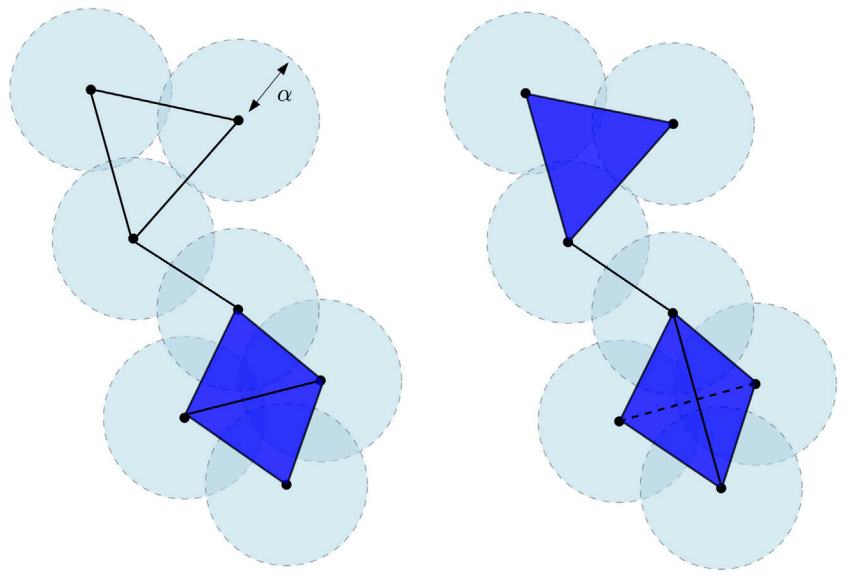
\includegraphics[width=0.85\linewidth]{./figures/Figura2_c1.png}
    \caption{
        El complejo de \v Cech, $Cech_{\alpha}\left(\mathbb{X}\right)$ (izquierda) y el de Vietoris-Rips
        $Rips_{2\alpha}\left(\mathbb{X}\right)$ (derecha) en una nube finita de puntos en
        $\mathbb{R}^{2}$. La parte inferior de $Cech_{\alpha}\left(\mathbb{X}\right)$ es la uni\'on de
        dos tri\'angulos adyacentes, mientras que la parte inferior de
        $Rips_{2\alpha}\left(\mathbb{X}\right)$ es el tetraedro generado por los cuatro v\'ertices
        y todas sus caras. La dimensi\'on del complejo de \v Cech es $2$. La dimensi\'on del complejo
        de Vietoris-Rips es $3$. Es de notar que el complejo de Vietoris-Rips, en este caso, no puede ser inmerso en $\mathbb{R}^{2}$.
    }
    \label{fig:Figura 2}
    \vspace{15pt}
\end{figure}

\section*{El Teorema del Nervio}

El complejo de \v Cech es un caso particular de una familia de complejos asociados con cubiertas. Dada
una cubierta $\mathcal{U}=\left(U_{i}\right)_{i\in I}$ de $\mathbb{M}$, conjunto de puntos en
$\mathbb{R}^{d}$, es decir, una familia de conjuntos $U_{i}$ tales que
$\mathbb{M}=\cup_{i\in I}U_{i}$, el nervio de $\mathcal{U}$ es el complejo simplicial
abstracto $C\left(\mathcal{U}\right)$ cuyos v\'ertices son los $U_{i}$'s y que cumple

\begin{equation*}
    \sigma = \left[U_{i_{0}}, \dots, U_{i_{k}}\right] \in C\left(\mathcal{U}\right)
    \text{ si y s\'olo si } \cap_{j=0}^{k}U_{i_{j}}\neq\varnothing.
\end{equation*}

Dada una cubierta de un conjunto de datos, donde cada conjunto de la cubierta es, por ejemplo, una
agrupaci\'on de los puntos de los datos que tienen ciertas propiedades en com\'un,
su nervio proporciona una descripci\'on combinatoria, compacta y global, de las relaciones
entre estos conjuntos a trav\'es de sus patrones de intersecci\'on. Ver Figura (\ref{fig:Figura 3}).

\begin{figure}[ht]
    \centering
    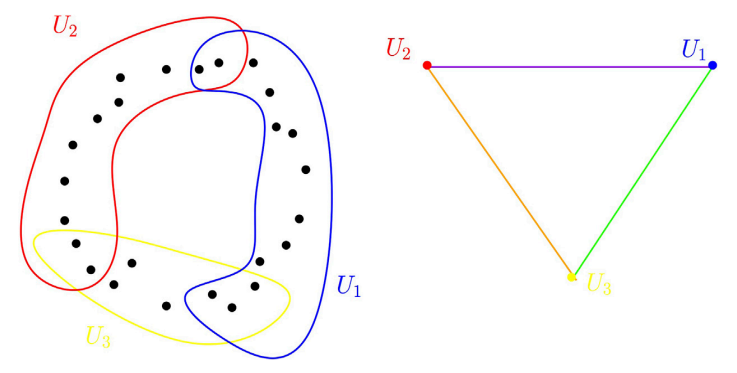
\includegraphics[width=0.85\linewidth]{./figures/Figura3.png}
    \caption{
        Nube de puntos muestreada en el plano y una cubierta de conjuntos abiertos para esta
        nube (izquierda). El nervio de esta cubierta es un tri\'agulo (derecha).
        Los v\'ertices corresponden a uno de los conjuntos de la cubierta mientras que
        las aristas corresponden a una de las
        intersecciones no vac\'ias entre dos conjuntos de la cubierta.
    }
    \label{fig:Figura 3}
    \vspace{15pt}
\end{figure}

Un teorema fundamental en topolog\'ia algebraica se encarga de relacionar, bajo ciertas condiciones, la
topolog\'ia del nervio de una cubierta con la topolog\'ia de la uni\'on de los conjuntos
de dicha cubierta. Es necesario introducir algunas nociones adicionales para ser
formales a la hora de enunciar este
resultado conocido como el teorema del nervio.

Dos espacios topol\'ogicos, $X$ y $Y$, usualmente son considerados iguales desde un punto de vista
topol\'ogico si son homeomorfos, esto es, si existen dos funciones, biyectivas y continuas,
$f:X\rightarrow Y$ y $g:Y\rightarrow X$ tales que $f\circ g$ y $g\circ f$ son las funciones
identidad de $Y$ y $X$, respectivamente. En muchas ocasiones, pedir que $X$ y $Y$ sean
homeomorfos resulta ser una condici\'on demasiado fuerte para asegurar que $X$ y $Y$
compartan propiedades topol\'ogicas de inter\'es para el ATD.
Dos funciones continuas $f_{0}, f_{1}:X\rightarrow Y$ se dicen ser homot\'opicas
si existe una funci\'on continua $H:X\times\left[0, 1\right]\rightarrow Y$ tal que para
cualquier $x\in X$, $H\left(x, 0\right) = f_{0}\left(x\right)$ y $H\left(x, 1\right) = g\left(x\right)$.
Los espacios $X$ y $Y$ se dicen ser homot\'opicamente equivalentes si existen
dos funciones, $f:X\rightarrow Y$ y $g:Y\rightarrow X$, tales que $f\circ g$ y $g\circ f$ son
homot\'opicas a la func\'on identidad de $Y$ y $X$, respectivamente.
Las funciones $f$ y $g$ son llamadas homot\'opicamente equivalentes. La noci\'on de
equivalencia homot\'opica es m\'as d\'ebil que la de homeomorfismo; si $X$ y $Y$ son homeomorfos, entonces
son homot\'opicamente equivalentes, pero el rec\'iproco no es cierto. Sin embargo, espacios que son
homot\'opicamente equivalentes a\'un comparten muchos invariantes topol\'ogicos, como la conexidad por
caminos, los grupos de homotop\'ia y, en particular, tienen la misma homolog\'ia.

Un espacio se dice ser contra\'ible si es homot\'opicamente equivalente a un punto. Las bolas, y en
general los conjuntos convexos en $\mathbb{R}^{d}$, son ejemplos b\'asicos de espacios contra\'ibles.
Las cubiertas abiertas, para las cuales se tiene que todos sus elementos e intersecciones son
contra\'ibles, tienen la siguiente propiedad.

\begin{teorema}[Teorema del Nervio]\label{teoNervio}
    Sea $\mathcal{U} = \left(U_{i}\right)_{i\in I}$ una
    cubierta abierta de un espacio topol\'ogico $X$ tal que la intesecci\'on
    de cualquier subcolecci\'on de los $U_{i}$'s es contra\'ible o vac\'ia.
    Entonces, $X$ y el nervio $C\left(\mathcal{U}\right)$ son
    homot\'opicamente equivalentes.
\end{teorema}

Es f\'acil verificar que subconjuntos convexos de espacios euclidianos son contra\'ibles. Como
consecuencia, si $\mathcal{U} = \left(U_{i}\right)_{i\in I}$ es una colecci\'on de subconjuntos convexos
de $\mathbb{R}^{d}$, entonces $C\left(\mathcal{U}\right)$ y $\cup_{i\in I}U_{i}$ son homot\'opicamente
equivalentes. En particular, si $\mathbb{X}$ es un conjunto de puntos en $\mathbb{R}^{d}$, entonces el
complejo de \v Cech $Cech_{\alpha}\left(\mathbb{X}\right)$ es homot\'opicamente equivalente a la uni\'on
de bolas $\cup_{x\in\mathbb{X}}B\left(x, \alpha\right)$.

El teorema del nervio juega un papel fundamental en el ATD; proporciona una manera de codificar la
topolog\'ia de espacios continuos en estructuras combinatorias abstractas que se ajustan con facilidad
al dise\~{n}o de estructuras de datos y algoritmos efectivos.